% arara: pdflatex 
% arara: bibtex
% arara: pdflatex
% arara: pdflatex
% arara: clean: {extensions: [ aux, bbl, out, toc, blg, thm ]}

\documentclass[aspectratio=169]{beamer}

\makeatletter
\newskip\@bigflushglue \@bigflushglue = -100pt plus 1fil
\def\bigcenter{\trivlist \bigcentering\item\relax}
\def\bigcentering{\let\\\@centercr\rightskip\@bigflushglue%
\leftskip\@bigflushglue
\parindent\z@\parfillskip\z@skip}
\def\endbigcenter{\endtrivlist}
\makeatother


\usetheme[lightmode, showmaxslides]{pureminimalistic}
%darkmode
\usepackage[utf8]{inputenc}
\usepackage[T1]{fontenc}
\usepackage{tikz}

\usepackage{appendixnumberbeamer}
\renewcommand{\appendixname}{\texorpdfstring{\translate{appendix}}{appendix}}

% References
\usepackage[doi, natbibapa]{apacite}
\renewcommand\bibliographytypesize{\tiny}
\let\realcitep\citep
\renewcommand*{\citep}[1]{{\small\realcitep{#1}}}
\let\realcite\cite
\renewcommand*{\cite}[1]{{\small\realcite{#1}}}

% Change logo
\renewcommand{\logotitle}{\vspace*{-20mm}\hspace*{-10.1mm}\includegraphics%
  [width=\paperwidth]{header.jpeg}}
\renewcommand{\logoheader}{}
\renewcommand{\logoheader}{\vspace{0em}}
\renewcommand{\logofooter}{\includegraphics%
  [width=.4\linewidth]{neemsis.png}}

% Color text
\definecolor{darkgreen}{RGB}{80,151,68}
\definecolor{lightgreen}{RGB}{164,204,76}
\definecolor{brick}{RGB}{197,102,63}
\definecolor{lightgray}{HTML}{A9A9A9}
\definecolor{lightgray2}{RGB}{113,113,113}

% Mail address
\usepackage{hyperref}
\hypersetup{colorlinks,linkcolor={lightgray2},citecolor={darkgreen},urlcolor={darkgreen}}

% Math
\usepackage{graphicx}
\usepackage{amssymb,amsmath}
\usepackage{upgreek}

% Rupee 
\usepackage{tfrupee}

% Change page word
\renewcommand{\pageword}{}

% Table
\usepackage{array}
\usepackage{booktabs}

% Source for table
\newcommand{\sourcetab}[1]{\vspace{1mm} \caption{{\tiny\textbf{Source}: {#1}}}}
\newcommand{\sourcefig}[1]{\vspace{1mm} \caption{{\tiny\textbf{Source}: {#1}}}}

% For shrink
\usepackage{adjustbox}


%\renewcommand{\beamertextcolor}{}
%\renewcommand{\beamerbgcolor}{}
%\renewcommand{\beamerfootertextcolor}{}
\renewcommand{\beamertitlecolor}{brick}

% Icones
\usepackage{fontawesome}



% *****************************************************************
% Title
% *****************************************************************
\title[Plan de thèse]{\textsc{Dette, Personnalité et Mariage en Inde rurale} \\ Plan de thèse à partir des données RUME \& NEEMSIS}
\author[A. Natal]{\textcolor{darkgreen}{Arnaud Natal} \textcolor{lightgreen}{\scriptsize Univ. Bordeaux}}
\institute{| \small 20 octobre 2021} 


% ******************************************************************
\begin{document}
% has to be loaded outside of a frame to work!
\maketitle



% *******************
 \begin{frame}{Déroulement de la présentation}
   \tableofcontents
   + \faCommentsO ~Évolution de l'emploi entre 2010 et 2020-21
 \end{frame}
% *******************


\section{Contribution des traits de personnalité dans l'analyse de la dette individuelle}
% *******************
\begin{frame}{Comment les compétences cognitives et les traits de personnalité jouent sur l'endettement individuel ?}
    \begin{vfilleditems}
        \item[\faBook] Marché du travail, éducation \citep{Almlund2011}, finances des ménages \citep{Brown2014}. Dette en Inde \citep{Rajakumar2019, Guerin2014}. Inégalités de genre et de caste \citep{Sarkar2020}. 
        \item[\faDatabase] NEEMSIS-1 et NEEMSIS-2.
		\item[\faIndustry] Probit, MCO, quantiles et FE. Variables d'interraction.
		\item[\faGift] Rôle limité du cognitif. OP-EX et CO plutôt bien. Femmes dalits bloquées, hommes non-dalits plus hétérogènes.
    \end{vfilleditems}
\end{frame}
% *******************


% *******************
%\begin{frame}[plain, shrink=2]{Résultats}
%% Table generated by Excel2LaTeX from sheet 'Factor1-5'
\begin{table}[htbp]
  \centering
  \caption{Marginal effects of the probability of being in debt in 2020-21}
    \resizebox{\columnwidth}{!}{%
    \begin{tabular}{lcccccccccccc}
    \toprule
          & (1)   &       & \multicolumn{2}{c}{(2)} &       & \multicolumn{2}{c}{(3)} &       & \multicolumn{4}{c}{(4)} \\
\cmidrule{2-2}\cmidrule{4-5}\cmidrule{7-8}\cmidrule{10-13}          & ME/(t-stat) &       & ME/(t-stat) & ME/(t-stat) &       & ME/(t-stat) & ME/(t-stat) &       & ME/(t-stat) & ME/(t-stat) & ME/(t-stat) & ME/(t-stat) \\
          & All   &       & Male  & Female &       & MUC   & Dalits &       & MUC male & Dalits male & MUC female & Dalits female \\
    \midrule
    Factor 1 (std) & \cellcolor[rgb]{ 1,  1,  0}-0.033 &       & -0.010 & \cellcolor[rgb]{ 1,  1,  0}-0.048 &       & \cellcolor[rgb]{ 1,  1,  0}-0.081 & -0.000 &       & -0.049 & 0.011 & \cellcolor[rgb]{ 1,  1,  0}-0.111 & -0.003 \\
          & (-1.910) &       & (-0.353) & (-1.860) &       & (-2.997) & (-0.021) &       & (-1.267) & (0.285) & (-2.369) & (-0.111) \\
    Factor 2 (std) & 0.005 &       & \cellcolor[rgb]{ 1,  1,  0}0.045 & -0.046 &       & 0.026 & -0.011 &       & \cellcolor[rgb]{ 1,  1,  0}0.093 & -0.004 & \cellcolor[rgb]{ 1,  1,  0}-0.083 & -0.014 \\
          & (0.276) &       & (1.705) & (-1.605) &       & (1.026) & (-0.467) &       & (2.311) & (-0.104) & (-1.862) & (-0.410) \\
    Factor 3 (std) & -0.018 &       & -0.006 & -0.036 &       & -0.039 & -0.005 &       & -0.022 & -0.010 & \cellcolor[rgb]{ 1,  1,  0}-0.088 & 0.006 \\
          & (-1.035) &       & (-0.217) & (-1.386) &       & (-1.529) & (-0.233) &       & (-0.605) & (-0.268) & (-2.082) & (0.177) \\
    Factor 4 (std) & 0.002 &       & 0.017 & -0.016 &       & -0.023 & 0.012 &       & -0.034 & 0.055 & -0.045 & -0.023 \\
          & (0.096) &       & (0.672) & (-0.599) &       & (-0.871) & (0.550) &       & (-0.877) & (1.523) & (-0.960) & (-0.761) \\
    Factor 5 (std) & -0.026 &       & -0.035 & -0.028 &       & -0.045 & -0.016 &       & -0.062 & -0.021 & -0.053 & -0.026 \\
          & (-1.446) &       & (-1.347) & (-1.042) &       & (-1.618) & (-0.680) &       & (-1.604) & (-0.605) & (-1.154) & (-0.788) \\
    Literacy & 0.019 &       & -0.001 & \cellcolor[rgb]{ 1,  1,  0}0.047 &       & 0.027 & 0.011 &       & 0.018 & -0.016 & 0.052 & 0.050 \\
          & (1.094) &       & (-0.039) & (1.976) &       & (1.237) & (0.491) &       & (0.603) & (-0.479) & (1.585) & (1.625) \\
    Numeracy & -0.006 &       & 0.002 & -0.025 &       & -0.011 & -0.002 &       & -0.037 & 0.033 & -0.006 & -0.037 \\
          & (-0.304) &       & (0.053) & (-0.837) &       & (-0.374) & (-0.075) &       & (-0.909) & (0.785) & (-0.134) & (-0.945) \\
    Raven & 0.001 &       & 0.002 & -0.002 &       & -0.002 & 0.003 &       & 0.000 & 0.006 & -0.004 & -0.000 \\
          & (0.239) &       & (0.708) & (-0.609) &       & (-0.567) & (0.928) &       & (0.102) & (1.106) & (-0.848) & (-0.103) \\

\cmidrule{1-2}\cmidrule{4-5}\cmidrule{7-8}\cmidrule{10-13}    Indebted (=1) in 2016-17 & 0.414 &       & \multicolumn{2}{c}{0.412} &       & \multicolumn{2}{c}{0.390} &       & \multicolumn{4}{c}{0.389} \\
          & (2.752) &       & \multicolumn{2}{c}{(2.719)} &       & \multicolumn{2}{c}{(2.563)} &       & \multicolumn{4}{c}{(2.523)} \\
    Debtor ratio in 2016-17 & -0.157 &       & \multicolumn{2}{c}{-0.165} &       & \multicolumn{2}{c}{-0.152} &       & \multicolumn{4}{c}{-0.144} \\
          & (-2.194) &       & \multicolumn{2}{c}{(-2.344)} &       & \multicolumn{2}{c}{(-2.141)} &       & \multicolumn{4}{c}{(-1.966)} \\
    Individuals controls & X     &       & \multicolumn{2}{c}{X} &       & \multicolumn{2}{c}{X} &       & \multicolumn{4}{c}{X} \\
    Households controls & X     &       & \multicolumn{2}{c}{X} &       & \multicolumn{2}{c}{X} &       & \multicolumn{4}{c}{X} \\
    Villages FE & X     &       & \multicolumn{2}{c}{X} &       & \multicolumn{2}{c}{X} &       & \multicolumn{4}{c}{X} \\
    \midrule
    Observations & 831   &       & \multicolumn{2}{c}{831} &       & \multicolumn{2}{c}{831} &       & \multicolumn{4}{c}{831} \\
    Pseudo $R^2$ & 0.205 &       & \multicolumn{2}{c}{0.218} &       & \multicolumn{2}{c}{0.214} &       & \multicolumn{4}{c}{0.236} \\
    Log-likelihood & -387.994 &       & \multicolumn{2}{c}{-381.828} &       & \multicolumn{2}{c}{-383.822} &       & \multicolumn{4}{c}{-373.271} \\
    $\upchi^2$ & 240.884 &       & \multicolumn{2}{c}{246.493} &       & \multicolumn{2}{c}{326.328} &       & \multicolumn{4}{c}{314.239} \\
    p-value & 0.000 &       & \multicolumn{2}{c}{0.000} &       & \multicolumn{2}{c}{0.000} &       & \multicolumn{4}{c}{0.000} \\
    \bottomrule

    \end{tabular}%
	}
  \label{tab:ame_indebt}%
  \sourcetab{NEEMSIS-1 (2016-17) and NEEMSIS-2 (2020-21); author's calculations.}
\end{table}%
%\end{frame}
% *******************




\section{Analyse de l'évolution des traits de personnalité dans le temps}
% *******************
\begin{frame}{Les traits de personnalité sont-ils stables dans le temps ?}
    \begin{vfilleditems}
        \item[\faBook] Stable dans le temps \citep{CobbClark2012}. Pas de consensus en psychologie \citep{Ardelt2000}. Big-5 peu adapté au PED \citep{Laajaj2019}. 
        \item[\faDatabase] NEEMSIS-1 et NEEMSIS-2.
		\item[\faIndustry] Statistiques descriptives, MCO, FE.
		\item[\faGift] Instabilité dans le temps.
    \end{vfilleditems}
\end{frame}
% *******************


% *******************
\begin{frame}[plain, shrink=1]{Questions du Big-5 \& corr. biais}
% Table generated by Excel2LaTeX from sheet 'Factor1-5'
\begin{table}[htbp]
  \centering
  \caption{Details for personality test questions}
  \resizebox{\columnwidth}{!}{%
    \begin{tabular}{llc}
    \toprule
    Variable & Question & Big-5 traits  \\
    \midrule
    curious & Are you curious, interested in learning new things? & OP     \\
    interestbyart & Are you interested in nature, art or music? & OP     \\
    repetitivetasks & Do you prefer work that involves repetitive tasks and routines? & OP    \\
    inventive & Are you inventive, and discover new ways of doing things? & OP    \\
    liketothink & Do you like to think a lot, and reflect about ideas? & OP    \\
    newideas & Do you come up with original or new ideas? & OP  \\
    activeimagination & Do you have an active imagination? & OP   \\
    organized & Are you organized? & CO   \\
    makeplans & Do you make plans and stick to them? & CO \\
    workhard & Do you work hard to do things well and on time? & CO    \\
    appointmentontime & Do you get to work and appointments on time? & CO   \\
    putoffduties & Do you put off your duties in order to relax? & CO   \\
    easilydistracted & Do you get easily distracted? & CO   \\
    completeduties & Do you complete your duties on time? & CO   \\
    enjoypeople & Do you enjoy being with people? & EX  \\
    sharefeelings & Do you easily share your thoughts and feelings with other people? & EX  \\
    shywithpeople & Are you shy with people? & EX   \\
    enthusiastic & Are you enthusiastic and full of energy? & EX   \\
    talktomanypeople & In social gatherings, do you like to talk to many people? & EX   \\
    talkative & Are you talkative? & EX  \\
    expressedthoughts & Are you comfortable expressing your thoughts and opinions to others? & EX \\
    workwithother & Do you work well with other people? & AG   \\
    understandotherfeeling & Do you try to understand how other people feel and think? & AG  \\
    trustingofother & Are you generally trusting of other people? & AG  \\
    rudetoother & Do you tend to be rude to other people? & AG   \\
    toleratefaults & Do you tolerate faults in other people? & AG   \\
    forgiveother & Do you forgive other people easily? & AG   \\
    helpfulwithothers & Are you helpful with others? & AG  \\
    managestress & Do you manage stress well? & ES   \\
    nervous & Do you get nervous easily? & ES  \\
    changemood & Do you have sudden changes in your mood? & ES   \\
    feeldepressed & Do you feel sad, depressed? & ES   \\
    easilyupset & Do you get easily upset? & ES   \\
    worryalot & Do you worry a lot? & ES   \\
    staycalm & Do you stay calm in tense or stressful situations? & ES  \\
    \bottomrule
    \end{tabular}%
	}
  \label{tab:big5}%
  \sourcetab{NEEMSIS-1 (2016-17) \& NEEMSIS-2 (2020-21)}
\end{table}%

\end{frame}
% *******************



% *******************
\begin{frame}[plain, shrink=2]{Correction 1 \citep{Rammstedt2013}}
\begin{figure}[htpb]
\centering
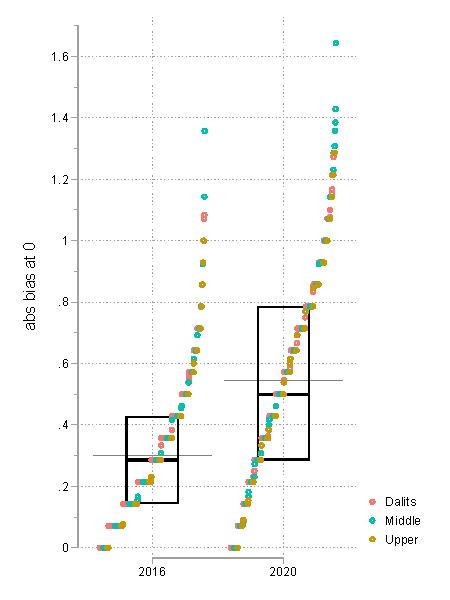
\includegraphics[scale=1]{INPUT/boxplotars.pdf}
\end{figure}
\end{frame}
% *******************



% *******************
\begin{frame}[plain, shrink=2]{Correction 2 "maison"}
\begin{figure}[H]
    \centering
    \begin{columns}[T]
        \begin{column}{.5\linewidth}
            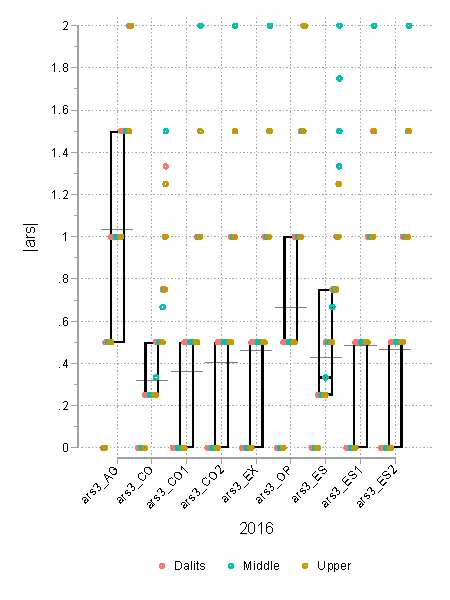
\includegraphics[width=\linewidth]{INPUT/boxplotars2016_det.pdf}
        \end{column}
        \begin{column}{.5\linewidth}
            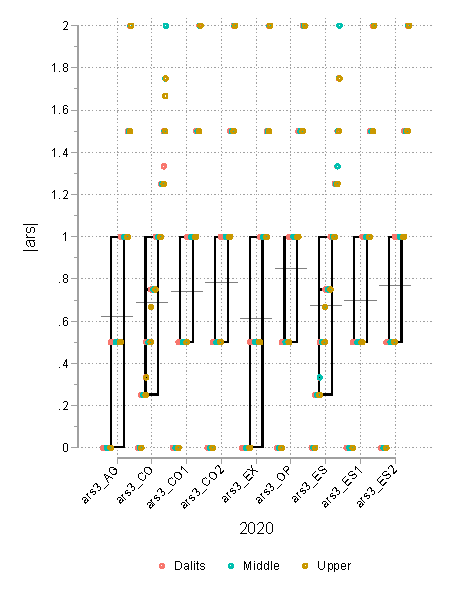
\includegraphics[width=\linewidth]{INPUT/boxplotars2020_det.pdf}
        \end{column}
    \end{columns}
\end{figure}
 \end{frame}
% *******************



% *******************
\begin{frame}[plain, shrink=2]{Rôle des enquêteurs en 2016-17}
% Table generated by Excel2LaTeX from sheet 'Traits2016'
\begin{table}[htbp]
  \centering
    \begin{tabular}{lccccccccccc}
    \toprule
      & 2016-17 &   & (1) & (2) & (3) & (4) & (5) & (6) & (7) & (8) & (9) \\
      & AB &   & AG & CO & CO1 & CO2 & EX & OP & ES & ES1 & ES2 \\
      & b/se &   & b/se & b/se & b/se & b/se & b/se & b/se & b/se & b/se & b/se \\
    \midrule
    Antoni & 0.000 &   & 0.000 & 0.000 & 0.000 & 0.000 & 0.000 & 0.000 & 0.000 & 0.000 & 0.000 \\
      & (.) &   & (.) & (.) & (.) & (.) & (.) & (.) & (.) & (.) & (.) \\
    Antoni - Vivek Radja & 0.020 &   & -0.176 & -0.121 & -0.266 & -0.070 & 0.238 & 0.023 & 0.146 & 0.070 & 0.191 \\
      & (0.141) &   & (0.304) & (0.183) & (0.240) & (0.265) & (0.282) & (0.345) & (0.231) & (0.284) & (0.278) \\
    Kumaresh & 0.056 &   & 0.312*** & 0.106** & 0.147** & 0.180*** & 0.238*** & 0.298*** & 0.051 & 0.058 & 0.141** \\
      & (0.036) &   & (0.077) & (0.047) & (0.061) & (0.067) & (0.072) & (0.088) & (0.059) & (0.072) & (0.071) \\
    Kumaresh - Raja Annamalai & -0.123 &   & 0.574* & 0.129 & 0.234 & -0.070 & -0.262 & 0.773** & 0.146 & 0.070 & 0.691** \\
      & (0.141) &   & (0.304) & (0.183) & (0.240) & (0.265) & (0.282) & (0.345) & (0.231) & (0.284) & (0.278) \\
    Kumaresh - Sithanantham & 0.055 &   & 0.449** & 0.066 & 0.109 & -0.070 & 0.238 & 0.148 & -0.041 & -0.055 & -0.059 \\
      & (0.101) &   & (0.216) & (0.131) & (0.171) & (0.189) & (0.201) & (0.246) & (0.165) & (0.203) & (0.198) \\
    Mayan & 0.062** &   & 0.376*** & 0.087*** & 0.159*** & 0.121*** & 0.307*** & -0.049 & -0.052 & -0.019 & 0.060 \\
      & (0.024) &   & (0.052) & (0.031) & (0.041) & (0.045) & (0.048) & (0.059) & (0.039) & (0.048) & (0.047) \\
    Mayan - Raja Annamalai & 0.092 &   & 0.241 & 0.046 & 0.234* & -0.070 & 0.405** & 0.107 & -0.159 & -0.180 & 0.025 \\
      & (0.083) &   & (0.178) & (0.108) & (0.141) & (0.155) & (0.165) & (0.203) & (0.136) & (0.167) & (0.163) \\
    Pazhani & -0.031 &   & 0.543*** & 0.102*** & 0.284*** & -0.015 & 0.112** & 0.668*** & 0.339*** & 0.209*** & 0.522*** \\
      & (0.023) &   & (0.050) & (0.030) & (0.040) & (0.044) & (0.047) & (0.057) & (0.038) & (0.047) & (0.046) \\
    Raja Annamalai & 0.156*** &   & -0.006 & 0.252*** & 0.224*** & 0.297*** & 0.451*** & 0.311*** & 0.146*** & 0.182*** & 0.218*** \\
      & (0.027) &   & (0.058) & (0.035) & (0.046) & (0.051) & (0.054) & (0.066) & (0.044) & (0.054) & (0.053) \\
    Raja Annamalai - Pazhani & 0.234* &   & 0.824*** & 0.379** & 0.734*** & 0.430 & -0.012 & 0.023 & 0.021 & 0.070 & -0.059 \\
      & (0.141) &   & (0.304) & (0.183) & (0.240) & (0.265) & (0.282) & (0.345) & (0.231) & (0.284) & (0.278) \\
    Sithanantham & 0.256*** &   & 0.791*** & 0.050* & -0.009 & 0.125*** & 0.251*** & 0.145*** & 0.110*** & 0.151*** & 0.147*** \\
      & (0.023) &   & (0.049) & (0.029) & (0.038) & (0.042) & (0.045) & (0.055) & (0.037) & (0.046) & (0.045) \\
    Sithanantham - Raja Annamalai & 0.243*** &   & 0.449*** & 0.098 & 0.109 & -0.008 & 0.301** & 0.273 & 0.240** & 0.195 & 0.254* \\
      & (0.072) &   & (0.155) & (0.094) & (0.123) & (0.136) & (0.144) & (0.177) & (0.118) & (0.145) & (0.142) \\
    Vivek Radja & -0.054** &   & 0.141*** & -0.010 & -0.068* & 0.040 & 0.089* & -0.011 & -0.110*** & -0.215*** & -0.023 \\
      & (0.024) &   & (0.051) & (0.031) & (0.041) & (0.045) & (0.048) & (0.059) & (0.039) & (0.048) & (0.047) \\
    Vivek Radja - Mayan & 0.136*** &   & 0.185* & 0.046 & 0.040 & 0.069 & 0.322*** & 0.357*** & 0.082 & 0.043 & 0.136 \\
      & (0.050) &   & (0.107) & (0.065) & (0.085) & (0.094) & (0.100) & (0.122) & (0.082) & (0.100) & (0.098) \\
    Vivek Radja - Raja Annamalai & -0.088 &   & -0.176 & 0.004 & 1.234*** & 0.680* & 0.238 & 0.023 & 0.146 & 1.070*** & 0.191 \\
      & (0.199) &   & (0.428) & (0.258) & (0.339) & (0.374) & (0.397) & (0.487) & (0.326) & (0.401) & (0.392) \\
    constant & 0.230*** &   & 0.676*** & 0.246*** & 0.266*** & 0.320*** & 0.262*** & 0.477*** & 0.354*** & 0.430*** & 0.309*** \\
      & (0.018) &   & (0.038) & (0.023) & (0.030) & (0.033) & (0.035) & (0.043) & (0.029) & (0.035) & (0.035) \\
    \midrule
    Observations & 952 &   & 952 & 952 & 952 & 952 & 952 & 952 & 952 & 952 & 952 \\
    $R^2$ & 0.252 &   & 0.319 & 0.079 & 0.143 & 0.064 & 0.107 & 0.213 & 0.174 & 0.121 & 0.184 \\
    Adjusted $R^2$ & 0.241 &   & 0.309 & 0.065 & 0.130 & 0.050 & 0.093 & 0.201 & 0.161 & 0.108 & 0.172 \\
    p-value & 0.000 &   & 0.000 & 0.000 & 0.000 & 0.000 & 0.000 & 0.000 & 0.000 & 0.000 & 0.000 \\
    \bottomrule
    \end{tabular}%
\end{table}%

\end{frame}
% *******************



% *******************
\begin{frame}[plain, shrink=2]{Rôle des enquêteurs en 2020-21}
% Table generated by Excel2LaTeX from sheet 'Traits2020'
\begin{table}[htbp]
  \centering
    \begin{tabular}{lcrccccccccc}
    \toprule
      & 2020-21 &   & (1) & (2) & (3) & (4) & (5) & (6) & (7) & (8) & (9) \\
      & AB &   & AG & CO & CO1 & CO2 & EX & OP & ES & ES1 & ES2 \\
      & b/se &   & b/se & b/se & b/se & b/se & b/se & b/se & b/se & b/se & b/se \\
    \midrule
    Antoni & 0.000 &   & 0.000 & 0.000 & 0.000 & 0.000 & 0.000 & 0.000 & 0.000 & 0.000 & 0.000 \\
      & (.) &   & (.) & (.) & (.) & (.) & (.) & (.) & (.) & (.) & (.) \\
    Chithra-Radhika & 0.197*** &   & 0.132 & 0.292*** & 0.204* & 0.418*** & 0.210* & 0.447*** & 0.281*** & 0.387*** & 0.138 \\
      & (0.073) &   & (0.113) & (0.100) & (0.120) & (0.119) & (0.114) & (0.124) & (0.098) & (0.117) & (0.118) \\
    Mayan & 0.125* &   & 0.249** & 0.143 & 0.115 & 0.107 & 0.166 & 0.114 & 0.051 & 0.111 & -0.026 \\
      & (0.073) &   & (0.114) & (0.101) & (0.121) & (0.119) & (0.115) & (0.125) & (0.098) & (0.118) & (0.119) \\
    Pazani & 0.016 &   & 0.002 & 0.079 & 0.150 & -0.025 & 0.132 & 0.439*** & 0.037 & 0.052 & 0.020 \\
      & (0.078) &   & (0.122) & (0.108) & (0.129) & (0.127) & (0.123) & (0.133) & (0.105) & (0.126) & (0.127) \\
    Raichal & -0.147* &   & 0.210* & 0.062 & 0.210* & 0.160 & 0.461*** & 0.294** & 0.042 & 0.313** & 0.082 \\
      & (0.076) &   & (0.119) & (0.105) & (0.127) & (0.125) & (0.121) & (0.130) & (0.103) & (0.124) & (0.124) \\
    Rajalakschmi & 0.029 &   & 0.327*** & 0.165 & 0.207* & 0.269** & 0.274** & 0.259** & 0.049 & 0.261** & 0.069 \\
      & (0.075) &   & (0.117) & (0.104) & (0.125) & (0.123) & (0.119) & (0.128) & (0.101) & (0.122) & (0.122) \\
    Suganya-Malarvizhi & 0.152** &   & -0.021 & 0.216** & 0.167 & 0.247** & 0.313*** & 0.342*** & 0.202** & 0.239** & 0.162 \\
      & (0.073) &   & (0.113) & (0.100) & (0.120) & (0.119) & (0.115) & (0.124) & (0.098) & (0.118) & (0.118) \\
    Vivek Radja & 0.039 &   & -0.155 & 0.079 & -0.017 & 0.037 & -0.038 & 0.055 & -0.092 & -0.087 & -0.170 \\
      & (0.074) &   & (0.115) & (0.102) & (0.122) & (0.121) & (0.117) & (0.126) & (0.099) & (0.119) & (0.120) \\
    constant & 0.446*** &   & 0.524*** & 0.512*** & 0.595*** & 0.571*** & 0.405*** & 0.571*** & 0.560*** & 0.500*** & 0.714*** \\
      & (0.071) &   & (0.110) & (0.097) & (0.117) & (0.115) & (0.112) & (0.120) & (0.095) & (0.114) & (0.115) \\
    \midrule
    Observations & 1660 &   & 1659 & 1660 & 1660 & 1660 & 1660 & 1659 & 1660 & 1658 & 1660 \\
    $R^2$ & 0.079 &   & 0.082 & 0.033 & 0.019 & 0.069 & 0.061 & 0.067 & 0.078 & 0.081 & 0.043 \\
    Adjusted $R^2$ & 0.075 &   & 0.078 & 0.029 & 0.015 & 0.065 & 0.057 & 0.063 & 0.074 & 0.077 & 0.039 \\
    p-value & 0.000 &   & 0.000 & 0.000 & 0.000 & 0.000 & 0.000 & 0.000 & 0.000 & 0.000 & 0.000 \\
    \bottomrule
    \end{tabular}%
\end{table}%

\end{frame}
% *******************


% *******************
\begin{frame}[plain, shrink=2]{Cohérence interne des données 1}
\begin{figure}[htpb]
\centering
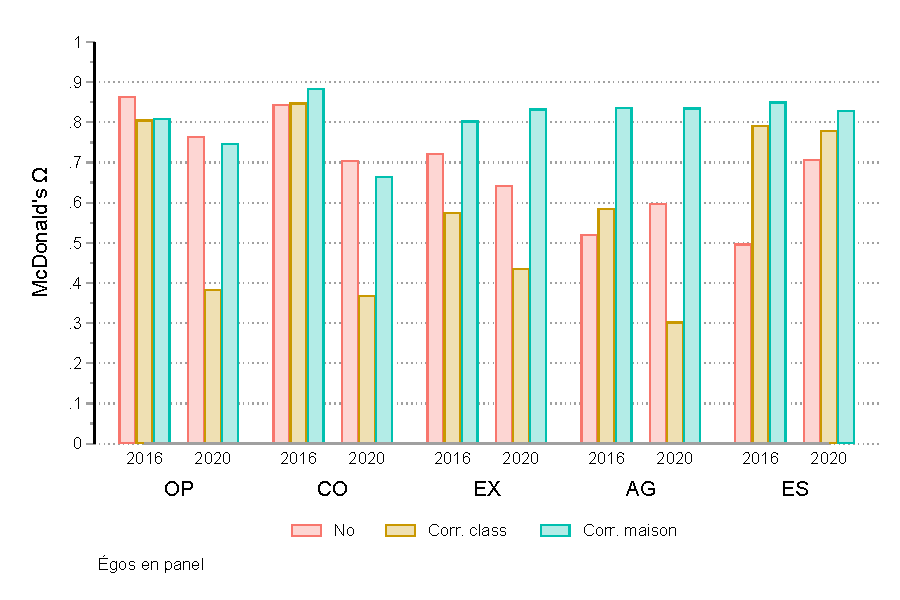
\includegraphics[scale=0.9]{INPUT/omega_panel.pdf}
\end{figure}
 \end{frame}
% *******************



% *******************
\begin{frame}[plain, shrink=2]{Cohérence interne des données 2}
\begin{figure}[htpb]
\centering
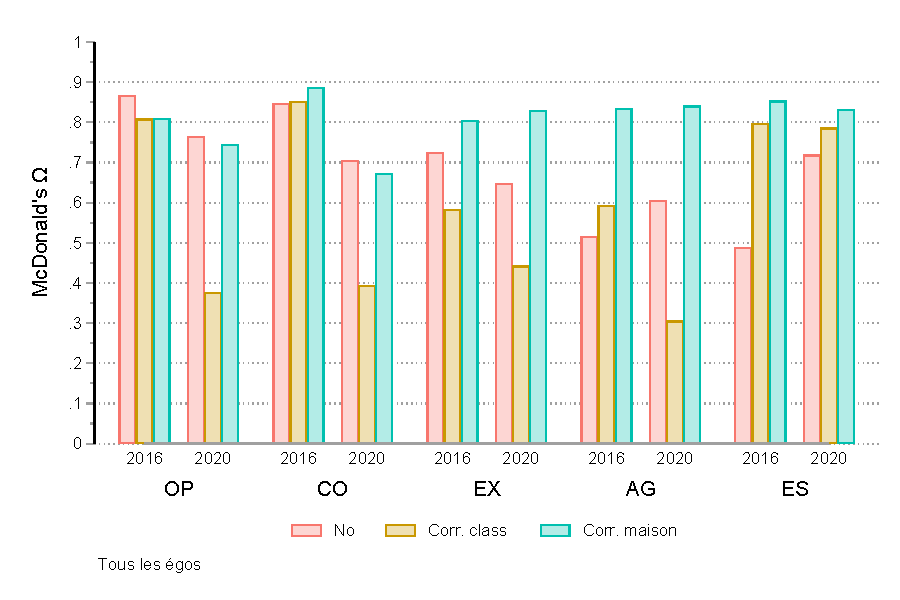
\includegraphics[scale=0.9]{INPUT/omega_tot.pdf}
\end{figure}
 \end{frame}
% *******************








\section{Persistence du surendettement des ménages}
% *******************
\begin{frame}{Quels sont les déterminants du surendettement des ménages ? Les trajectoires de surendettement ?}
    \begin{vfilleditems}
        \item[\faBook] Rôle du Covid-19 \citep{Guerin2021}. Persistance du surendettement \citep{Chichaibelu2018}.
        \item[\faDatabase] RUME, NEEMSIS-1 et NEEMSIS-2.
		\item[\faIndustry] Statistiques descriptives, FE (RE, CRE ?).
    \end{vfilleditems}
\end{frame}
% *******************







\section{Finances des mariages}
% *******************
\begin{frame}{Finances des mariages}
    \begin{vfilleditems}
        \item[\faBook] Gifts \citep{Bloch2004}.  \citep{Guerin2020c}.
        \item[\faDatabase] NEEMSIS-1, NEEMSIS-2 et enquêtes qualitatives.
		\item[\faIndustry] Statistiques descriptives, Statistique exploratoire multidimensionnelle (?). 
    \end{vfilleditems}
\end{frame}
% *******************






% *******************
\begin{frame}{\faCommentsO ~Évolution de l'emploi entre 2010 et 2020-21}
    \begin{vfilleditems}
        \item[2010] Agri; Coolie; Agri coolie; NREGS; Investment; Employee; SE; Pension.
        \item[2016] Agri; SE; SJ agri; SJ non-agri; UW in HH business; UW in other business; UW in own farm; UW in another farm.
        \item[2020] Agri; SE; SJ agri; SJ non-agri; UW in HH business; UW in other business; UW in own farm; UW in another farm.
        \item[Panel] Agri SE; Agri casual; Casual; Regular non-quali; Regular quali; SE; NREGA.
    \end{vfilleditems}
\end{frame}
% *******************



% *******************
\begin{frame}[plain, shrink=2]{Graphiques}
\begin{figure}[htpb]
\centering
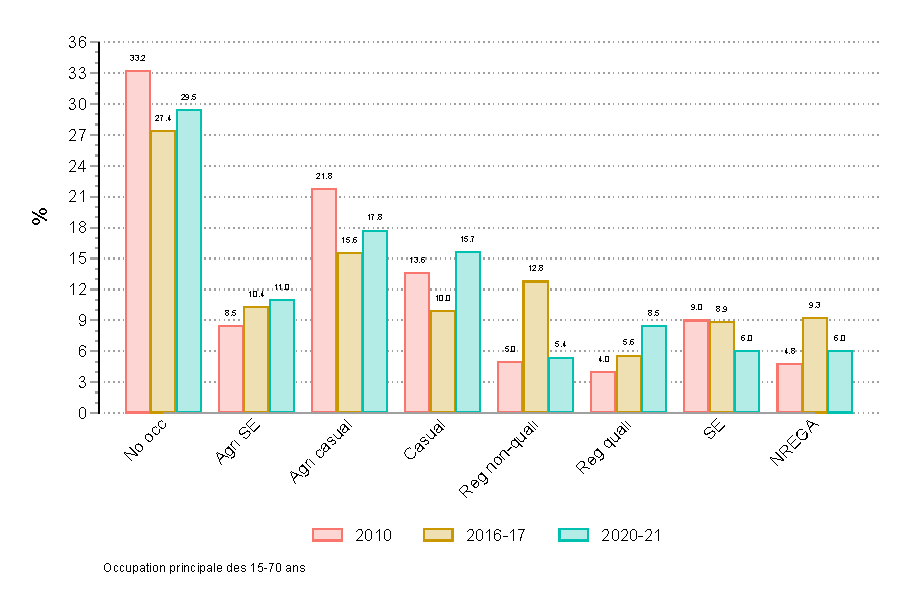
\includegraphics[scale=0.9]{INPUT/evo_moc_1570.pdf}
\end{figure}
\end{frame}
% *******************



% *******************
\begin{frame}[plain, shrink=2]{Graphiques}
\begin{figure}[htpb]
\centering
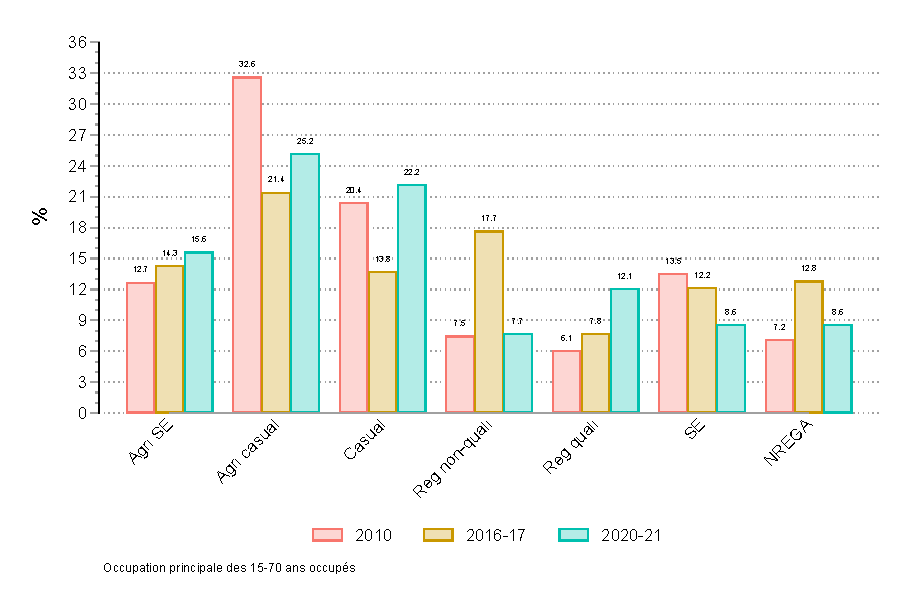
\includegraphics[scale=0.9]{INPUT/evo_moc_1570act.pdf}
\end{figure}
\end{frame}
% *******************


% *******************
\begin{frame}[plain, shrink=2]{Graphiques}
\begin{figure}[htpb]
\centering
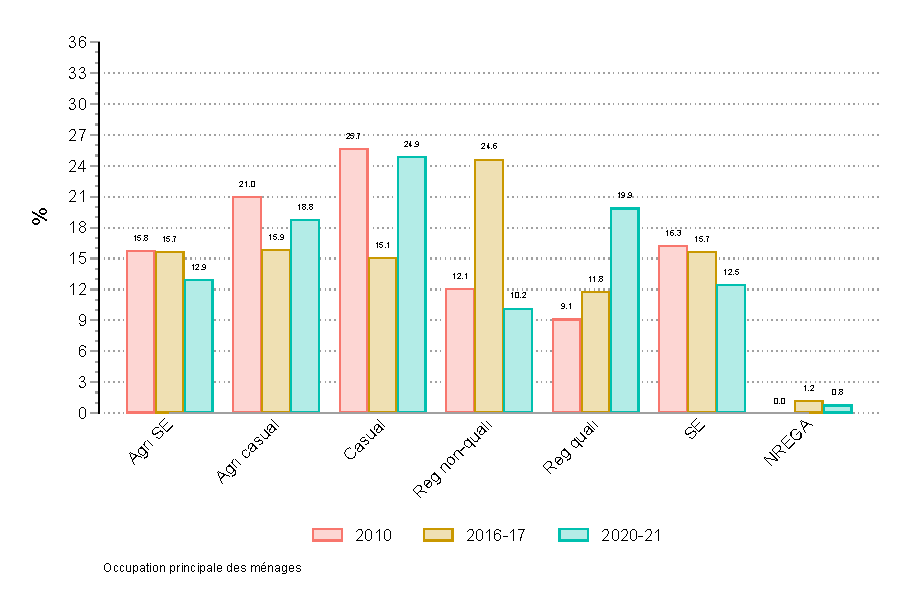
\includegraphics[scale=0.9]{INPUT/evo_moc_HH.pdf}
\end{figure}
\end{frame}
% *******************




% *******************
\begin{frame}[plain, shrink=2]{Graphiques}
\begin{figure}[htpb]
\centering
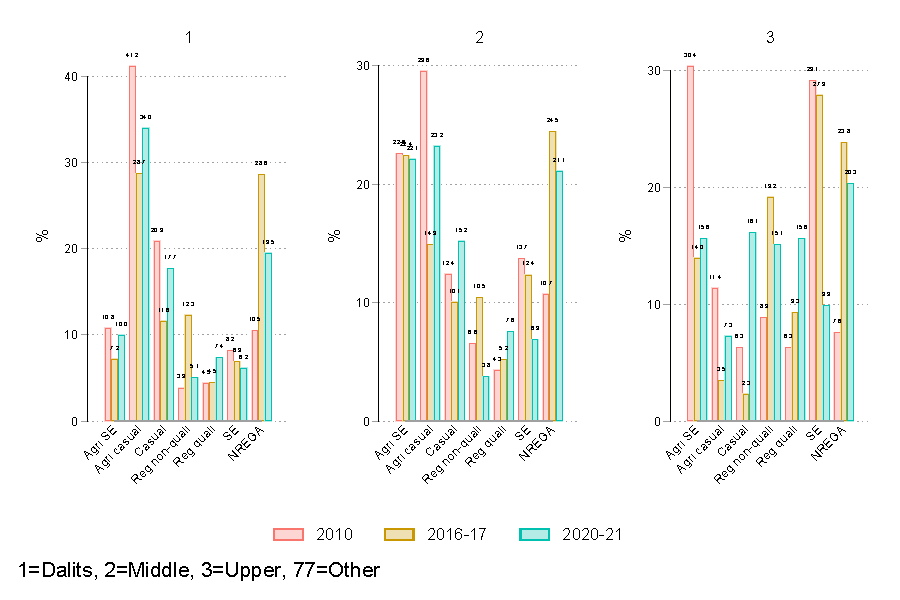
\includegraphics[scale=0.9]{INPUT/occ_year_caste.pdf}
\end{figure}
\end{frame}
% *******************



% *******************
\begin{frame}[plain, shrink=2]{Graphiques}
\begin{figure}[htpb]
\centering
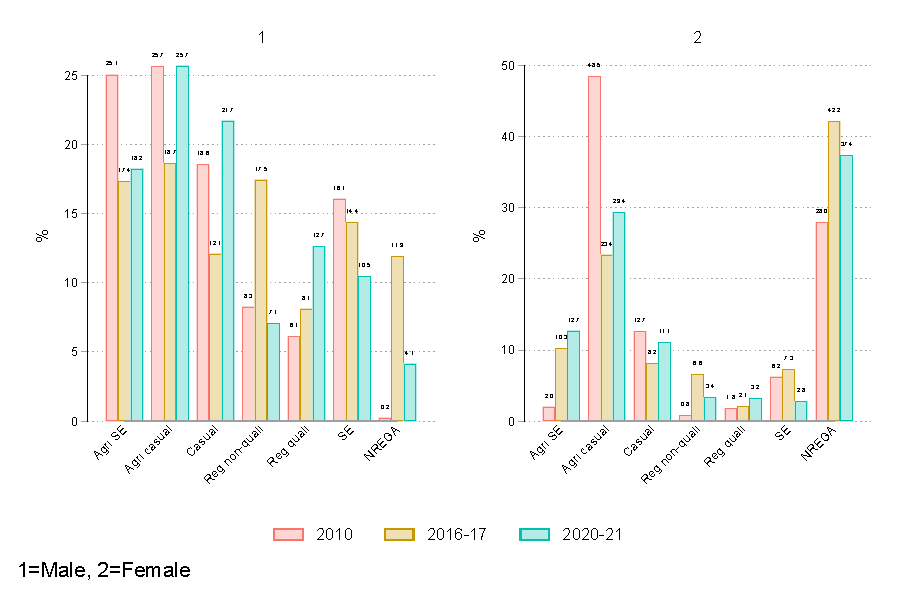
\includegraphics[scale=0.9]{INPUT/occ_year_sex.pdf}
\end{figure}
\end{frame}
% *******************





% *******************
\begin{frame}[plain, shrink=2]{Graphiques}
\begin{figure}[htpb]
\centering
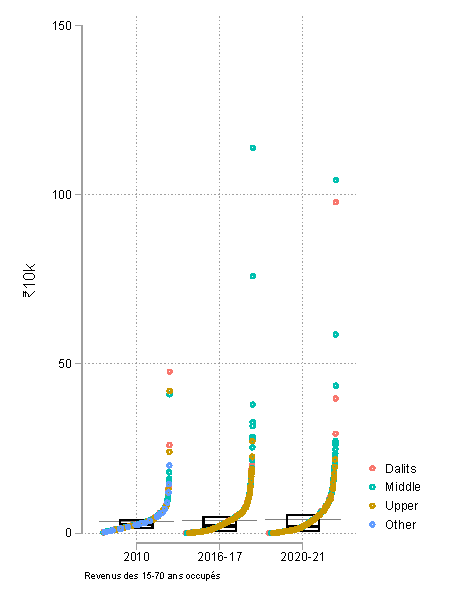
\includegraphics[scale=0.9]{INPUT/inc_indiv.pdf}
\end{figure}
\end{frame}
% *******************


% *******************
\begin{frame}[plain, shrink=2]{Graphiques}
\begin{figure}[htpb]
\centering
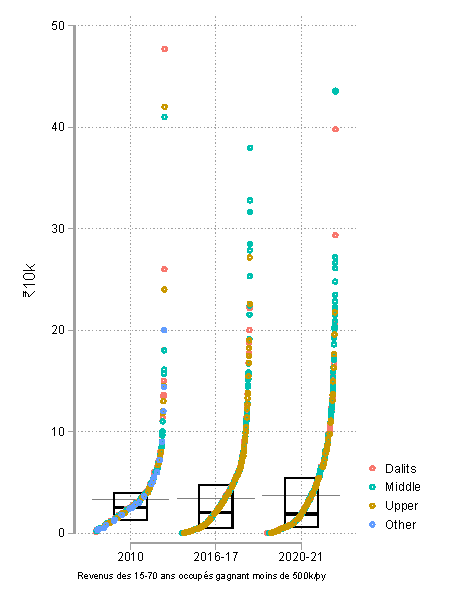
\includegraphics[scale=0.9]{INPUT/inc_indiv500k.pdf}
\end{figure}
\end{frame}
% *******************




% *******************
\begin{frame}[plain, shrink=2]{Graphiques}
\begin{figure}[htpb]
\centering
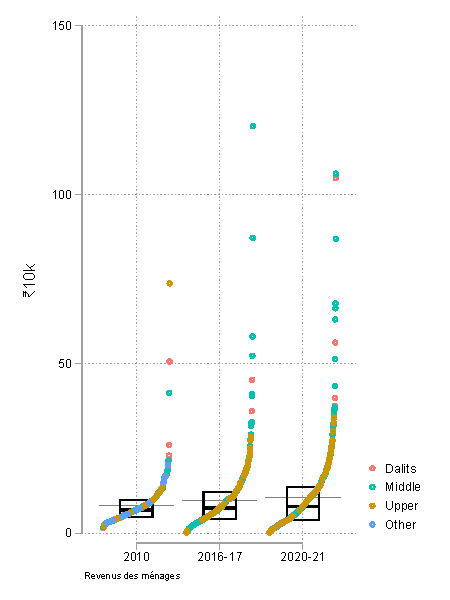
\includegraphics[scale=0.9]{INPUT/inc_hh.pdf}
\end{figure}
\end{frame}
% *******************


% *******************
\begin{frame}[plain, shrink=2]{Graphiques}
\begin{figure}[htpb]
\centering
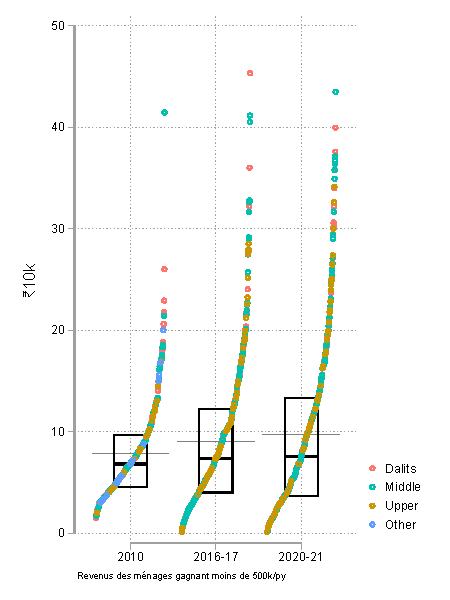
\includegraphics[scale=0.9]{INPUT/inc_hh500k.pdf}
\end{figure}
\end{frame}
% *******************




% *******************
\begin{frame}[plain, shrink=2]{Graphiques}
\begin{figure}[htpb]
\centering
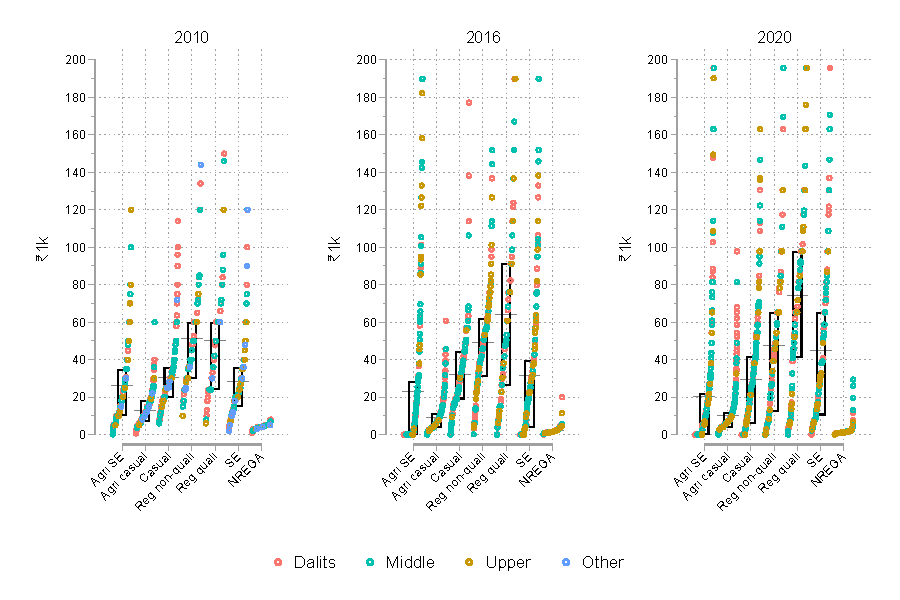
\includegraphics[scale=0.9]{INPUT/inc_occ_panel.pdf}
\end{figure}
\end{frame}
% *******************





% *******************
% \begin{frame}{Figures}
%     \begin{figure}[H]
%         \centering
%         \begin{columns}[T]
%             \begin{column}{.3\linewidth}
%                 \includegraphics[width=\linewidth]{example-image-a}
%                 \caption{Example A}
%             \end{column}
%             \begin{column}{.3\linewidth}
%                 \includegraphics[width=\linewidth]{example-image-b}
%                 \caption{Example B}
%             \end{column}
%         \end{columns}
%     \end{figure}
% \end{frame}
% *******************


% *******************
\section*{References}
\begin{frame}[noframenumbering, allowframebreaks]{References}
\bibliographystyle{apacite}
\bibliography{Ref_Arnaud}
\end{frame}
% *******************


\end{document}